\documentclass[letterpaper]{article}
\usepackage[submission]{aaai24}
\usepackage{times}  % DO NOT CHANGE THIS
\usepackage{helvet}  % DO NOT CHANGE THIS
\usepackage{courier}  % DO NOT CHANGE THIS
\usepackage[hyphens]{url}  % DO NOT CHANGE THIS
\usepackage{graphicx} % DO NOT CHANGE THIS
\urlstyle{rm} % DO NOT CHANGE THIS
\def\UrlFont{\rm}  % DO NOT CHANGE THIS
\usepackage{natbib}  % DO NOT CHANGE THIS AND DO NOT ADD ANY OPTIONS TO IT
\usepackage{caption} % DO NOT CHANGE THIS AND DO NOT ADD ANY OPTIONS TO IT
\frenchspacing  % DO NOT CHANGE THIS
\setlength{\pdfpagewidth}{8.5in} % DO NOT CHANGE THIS
\setlength{\pdfpageheight}{11in} % DO NOT CHANGE THIS
%\usepackage{latexsym}
\usepackage{subcaption}
%\usepackage{subfigure}
\usepackage{hhline}
\usepackage{booktabs}
\usepackage{multirow}
\usepackage{amsmath}
%\usepackage{graphicx}
%\usepackage{makecell}
%\usepackage{bm}
\usepackage{url}
\usepackage{float}
\let\Bbbk\relax
\usepackage{amssymb}
\usepackage{tabularx}
\usepackage{makecell}
\usepackage{multicol}
\usepackage[T1]{fontenc}
\usepackage[utf8]{inputenc}
\usepackage{microtype}
\usepackage{inconsolata}
\newcommand{\secref}[1]{Sec. \ref{#1}}
\newcommand{\figref}[1]{Figure \ref{#1}}
\newcommand{\eqnref}[1]{Eq. (\ref{#1})}
\newcommand{\tabref}[1]{Table \ref{#1}}
\newcommand{\exref}[1]{Example \ref{#1}}
\newcommand{\KZ}[1]{\textcolor{blue}{(Kenny: #1)}}
\newcommand{\MY}[1]{\textcolor{orange}{(Mengyue: #1)}}
\newcommand{\AT}[1]{\textcolor{red}{(Arthur: #1)}}
\newcommand{\CH}[1]{\textcolor{green}{(Chunhao: #1)}}
\newcommand{\JY}[1]{\textcolor{purple}{(Jieyi: #1)}}
\usepackage[ruled,linesnumbered]{algorithm2e}
\usepackage{newfloat}
\usepackage{listings}
\usepackage{tipa}


\DeclareCaptionStyle{ruled}{labelfont=normalfont,labelsep=colon,strut=off} % DO NOT CHANGE THIS
\lstset{%
        basicstyle={\footnotesize\ttfamily},% footnotesize acceptable for monospace
        numbers=left,numberstyle=\footnotesize,xleftmargin=2em,% show line numbers, remove this entire line if you don't want the numbers.
        aboveskip=0pt,belowskip=0pt,%
        showstringspaces=false,tabsize=2,breaklines=true}
\floatstyle{ruled}
\newfloat{listing}{tb}{lst}{}
\floatname{listing}{Listing}
\pdfinfo{
/TemplateVersion (2024.1)
}
\setcounter{secnumdepth}{2} %May be changed to 1 or 2 if section numbers are desired.

\title{Towards Lexical Analysis of Dog Vocalizations via Online Videos}
\begin{document}
\maketitle
\appendix

\section{Implementation details}
In this part, we explain our implementation details. For PANNs, we use the original model and predefined parameters to extract ``sentences''. Based on the ``framewise output'' of the output of the model, we decide whether to maintain this audio segment. For ``word segmentation'', we finetune a Cnn8-Rnn network using predefined architecture of PANNs model with pre-defined parameters. For ``subword extraction'', we change the parameters of the oscillator-based speech syllabification algorithm to make it suitable for dog sounds. For IPA vowel extraction, we collect three sets of IPA vowel sounds and use voice conversion to double the sets. Then we average the whisper feature for all 6 tracks for each ipa vowel. We calculate the Euclidien similarity between each subword and IPA vowel features to assign the most similar ipa symbol to each subword. 

In the part of ``surrounding context extraction'', when inferencing the location, we fine-tuned a Resnet50 from models pre-trained on Places365, then 5 frames are sampled uniformly from the period before and after the vocalization, and then the location category with the largest sum of logits is voted out as the final result for ``location''. As for the activity, we fine-tuned a model from TSN, then a 2-second video clip which contains 1 second before the vocalization and 1 second after the vocalization is sent to the video understanding model, and the result of the ``activity'' is inferenced based on this clip. 

The whole experiment is running on an Ubuntu system server with four 2080ti GPUs and 128G RAM. 

\section{Location and Activity Inference Error Analysis}

In this part, we will evaluate the methods we raised which can tell us where the dog is (location) and what the dog is doing (activity). 

To get the location from the video, we fine-tuned an image classification model and vote on 5 frame results to decide the location. 
The overall accuracy of this model is 77.99\%. ~\figref{fig:context evaluation 1} presents the confusion matrix of a test set result with 209 images, the unit of the number in each cell is one image sample. For most of the location classes, this model can precisely infer the location. There may be some confusion between categories, such as ``food'' and ``living room'', ``water'' and ``woods'', this may be due to the simultaneous appearance of the characteristics of multiple locations in the same picture. For the class ``cage'', the recall is a bit low from this confusion matrix. One possible reason is that there are only 4 samples from this category. From the further exploration of the dataset, the model can still distinguish ``cage'' from ``living room''. 

To get the activity from the video, we fine-tuned a video understanding model, and use the model to decide the dog activity based on a 2-seconds period of video. The overall accuracy of this model is 61.40\%. ~\figref{fig:context evaluation 2} presents the confusion matrix of a test set result with 513 videos on this model. There are some categories that can be confused with each other, like ``sit'' and ``mount or hump (beg)'', ``stand'' and ``walk'', ``play with people'' and ``be touched''. The reason that these pairs can lead to more confusion is that the activities themself are similar, this realization is reflected in the different performance of the model across categories. 


\begin{figure*}[htb]
	\centering
	\begin{subfigure}[]{0.4\textwidth}
		\centering
		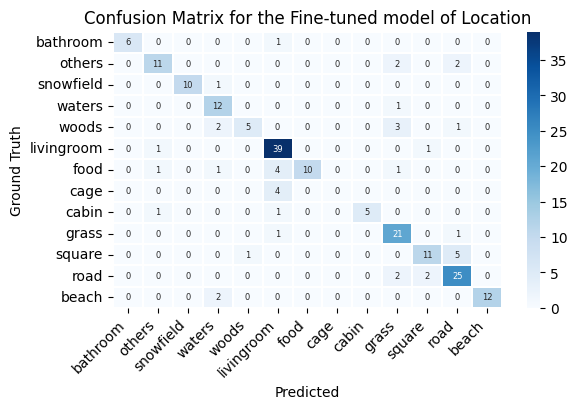
\includegraphics[width=0.9\textwidth]{images/location_cm.png}
		\caption{Location model confusion matrix.}
		\label{fig:context evaluation 1}
	\end{subfigure}
	\begin{subfigure}[]{0.4\textwidth}
		\centering
		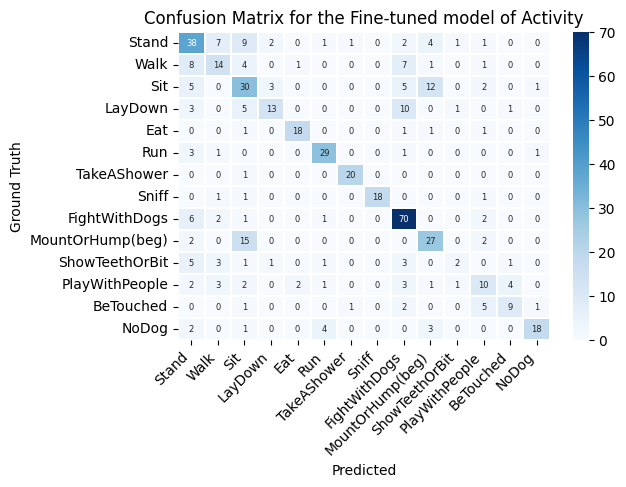
\includegraphics[width=0.9\textwidth]{images/activity_cm.png}
		\caption{Activity model confusion matrix.}
		\label{fig:context evaluation 2}
	\end{subfigure}
\caption{Context Evaluation.}
\label{fig:context evaluation}
\end{figure*}


\section{Details of Dataset}


\begin{table}[th]
\small
\centering
\begin{tabular}{p{0.3\columnwidth}|p{0.3\columnwidth}}
\toprule
\textbf{Word Type} & \textbf{Duration} \\
\hline
Whimper & 3.32 seconds \\
\hline
Yip & 0.36 seconds \\
\hline
Bow-wow & 0.28 seconds\\
\hline
Growl & 0.88 seconds \\
\hline
Bark & 0.4 seconds \\
\hline
Howl & 1.08 seconds \\
\bottomrule
\end{tabular}
\caption{Summary of duration for word types.}
\label{tab:duration}
\end{table}

We present the average duration and stand deviation of each ipa vowel symbol assigned to subwords in ~\tabref{tab:ipa_duration}. The duration of each ipa symbol in different word types varies from each other which is illustrated by time standard deviation. 
\begin{figure}[th]
\centering
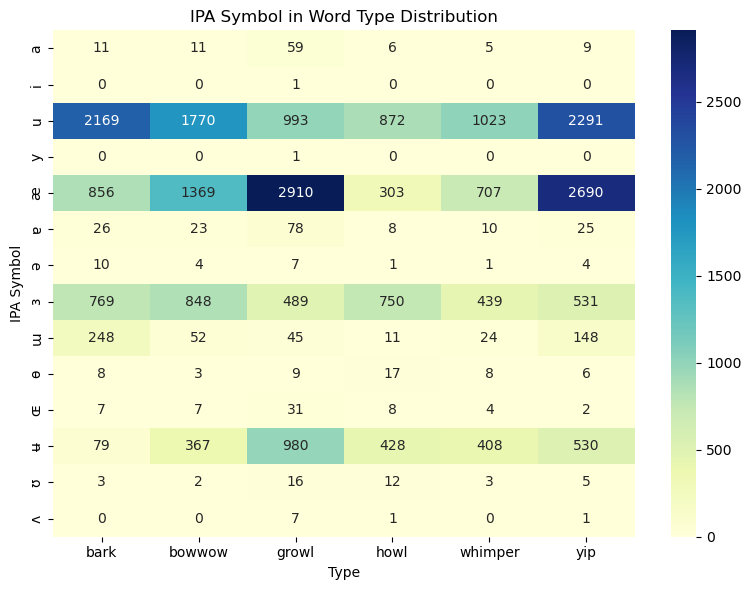
\includegraphics[width=0.8\columnwidth]{images/ipa_type_distri.png}
\caption{IPA symbol in word type distribution.} 
\label{fig:ipa_type_distri}
\end{figure}



\begin{table}[th]
\small
\centering
\begin{tabular}{p{0.2\columnwidth}|p{0.3\columnwidth}|p{0.4\columnwidth}}
\toprule
\textbf{IPA Vowel Symbol} & \textbf{Duration} & \textbf{Standard Deviation of Time Duration for Word Types} \\
\hline
u & 0.293 seconds & 0.0276 \\
\hline
\textrevepsilon & 0.213 seconds & 0.0312 \\
\hline
æ & 0.211 seconds & 0.0171\\
\hline
\textbaru & 0.233 seconds & 0.0152\\
\hline
\textturnm & 0.216 seconds & 0.0492\\
\hline
\textscoelig & 0.422 seconds & 0.0293\\
\hline
\textsci & 0.311 seconds & 0.0216\\
\hline
\textbaro & 0.479 seconds &0.0830\\
\hline
\textturna & 0.409 seconds &0.0217\\
\hline
a & 0.516 seconds & 0.0318 \\
\hline
\textschwa & 0.582 seconds & 0.0606 \\
\hline
\textturnv & 0.555 seconds & 0.0209\\
\hline
y & 0.528 seconds & 0 (only occurs one time)\\
\hline
i & 0.335 seconds & 0 (only occurs one time)\\
\bottomrule
\end{tabular}
\caption{Summary of duration and standard deviation for ipa vowel symbols.}
\label{tab:ipa_duration}
\end{table}

\section{Experiments for Analysing Subwords}

\begin{figure*}[h]
\centering
\begin{subfigure}[]{0.4\textwidth}
	\centering
	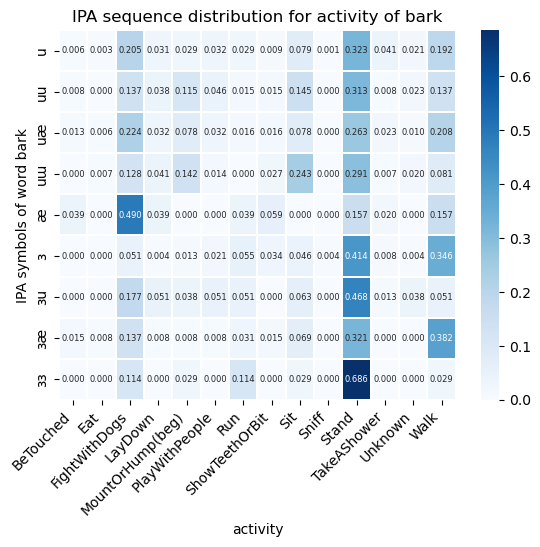
\includegraphics[width=0.9\textwidth]{images/ipa_bark.png}
	\caption{Activity distribution of subwords for bark.}
	\label{fig:1}
\end{subfigure}
\begin{subfigure}[]{0.4\textwidth}
	\centering
	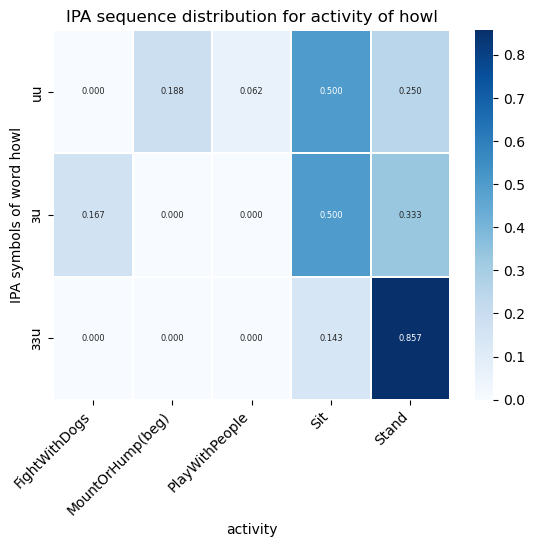
\includegraphics[width=0.9\textwidth]{images/ipa_howl.png}
	\caption{Activity distribution of subwords for howl.}
	\label{fig:2}
\end{subfigure}

\begin{subfigure}[]{0.4\textwidth}
	\centering
	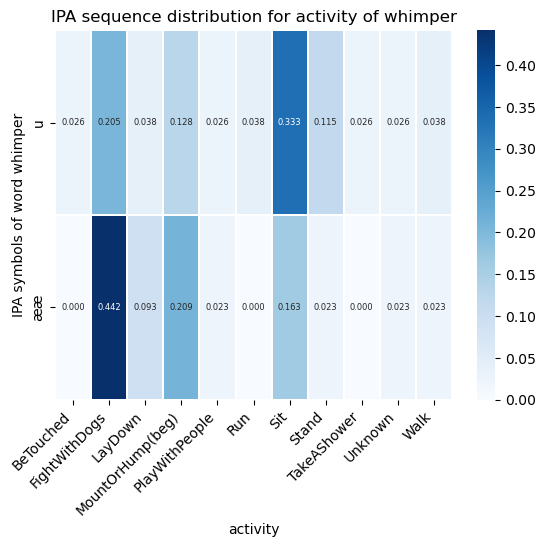
\includegraphics[width=0.9\textwidth]{images/ipa_whimper.png}
	\caption{Activity distribution of subwords for whimper.}
\label{fig:3}
\end{subfigure}
\begin{subfigure}[]{0.4\textwidth}
	\centering
	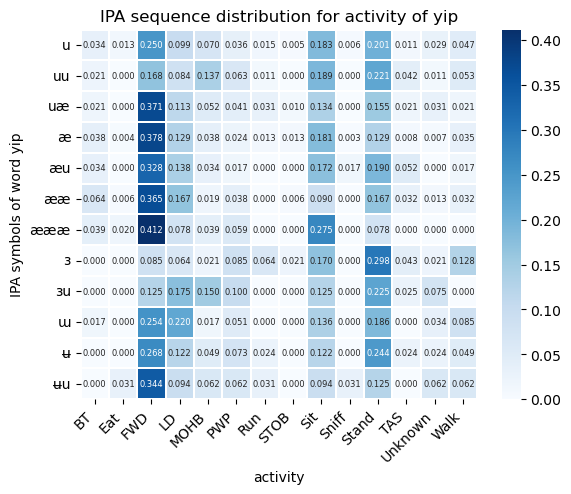
\includegraphics[width=0.9\textwidth]{images/output.png}
	\caption{Activity distribution of subwords for yip.}
\label{fig:4}
\end{subfigure}

\begin{subfigure}[]{0.4\textwidth}
	\centering
	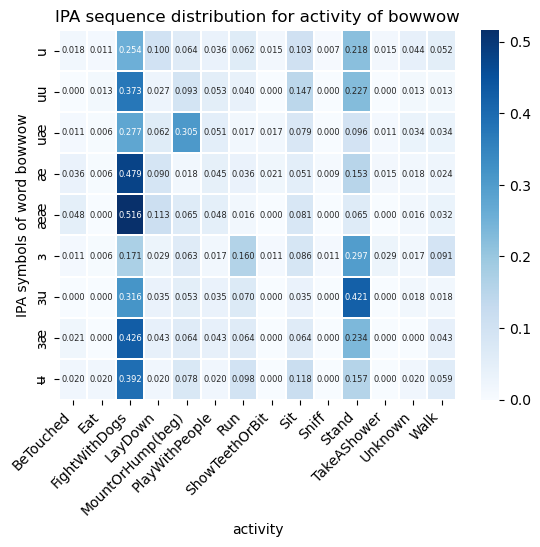
\includegraphics[width=0.9\textwidth]{images/ipa_bowwow.png}
	\caption{Activity distribution of subwords for bowwow.}
\label{fig:5}
\end{subfigure}
\begin{subfigure}[]{0.4\textwidth}
	\centering
	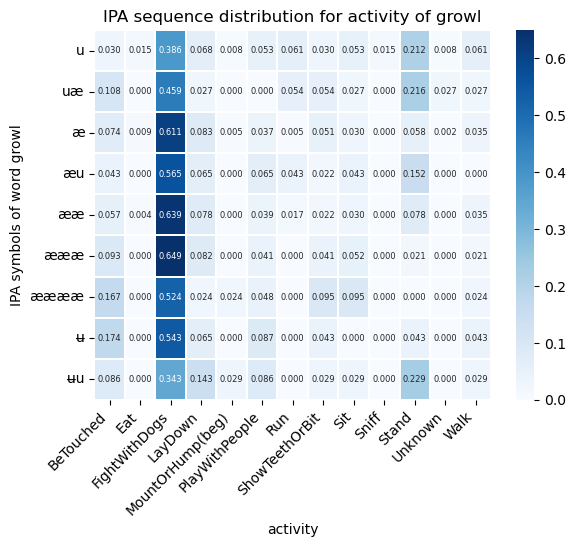
\includegraphics[width=0.9\textwidth]{images/ipa_growl.png}
	\caption{Activity distribution of subwords for growl.}
	\label{fig:6}
\end{subfigure}

\caption{Activity distribution of subwords.}
\label{fig:activity_subwords}
\end{figure*}



\begin{table}[t!]
\small
\centering
\begin{tabular}{p{0.45\columnwidth}|p{0.45\columnwidth}}
\toprule
\textbf{Word Type for Top 5 Frequent Subwords} & \textbf{Number of Dog Used} \\
\hline
Yip & 17.6 \\
\hline
Whimper & 9 \\
\hline
Howl & 4.25\\
\hline
Growl & 17 \\
\hline
Bowwow & 24.6 \\
\hline
Bark & 19.6 \\
\bottomrule
\end{tabular}
\caption{Summary to show frequent subwords are used by multiple dogs.}
\label{tab:subwords}
\end{table}

We collect the average number of different dogs using this subword for the 5 most frequent subwords of each word type in ~\tabref{tab:subwords}. ~\figref{fig:ipa_type_distri} shows the number of IPA symbols in different word types.
In order to prove that a word type can be further divided into more fine-grained types, for each word type, we collect the activity distribution of its IPA transcript which is a sequence of ipa symbols assigned to subwords. We find that the data distribution of word type ipa transcript can be mainly divided into several types, as they show an incoherent distribution for activities which implies in the same word type, these subparts convey different semantics. This shows that these words can be further divided into several different types. ~\figref{fig:activity_subwords} present the activity distribution for frequent ipa transcript for each word type as it is more intuitive using activity. 

If the subword conveys semantics, we can observe that these IPA symbols should present a different context distribution compared with word distribution.   For further analysis, we present IPA symbol distribution of activity for each word type in ~\figref{fig:activity_symbol_word_type}. We use activity instead of context and simply plot the number of coexistence instead of normalizing for clearness. 

\begin{figure*}[h]
\centering
\begin{subfigure}[]{0.4\textwidth}
	\centering
	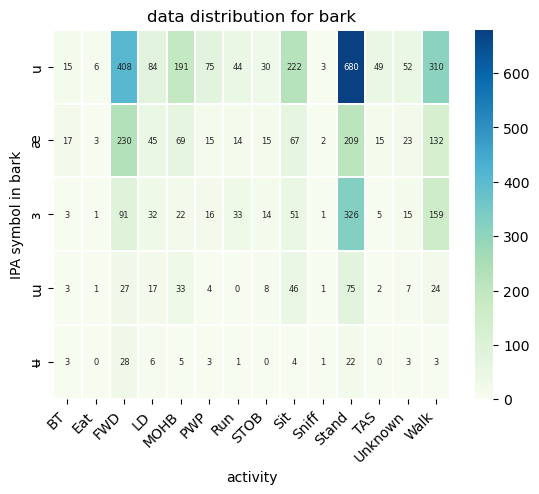
\includegraphics[width=0.9\textwidth]{images/symbol_bark.png}
	\caption{Activity distribution of subwords for bark.}
	\label{fig:11}
\end{subfigure}
\begin{subfigure}[]{0.4\textwidth}
	\centering
	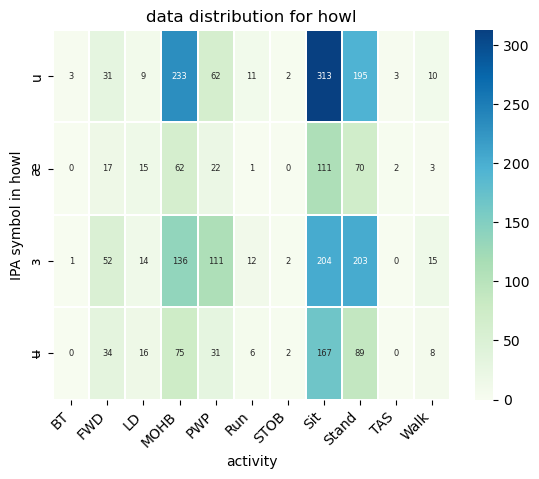
\includegraphics[width=0.9\textwidth]{images/symbol_howl.png}
	\caption{Activity distribution of subwords for howl.}
	\label{fig:21}
\end{subfigure}

\begin{subfigure}[]{0.4\textwidth}
	\centering
	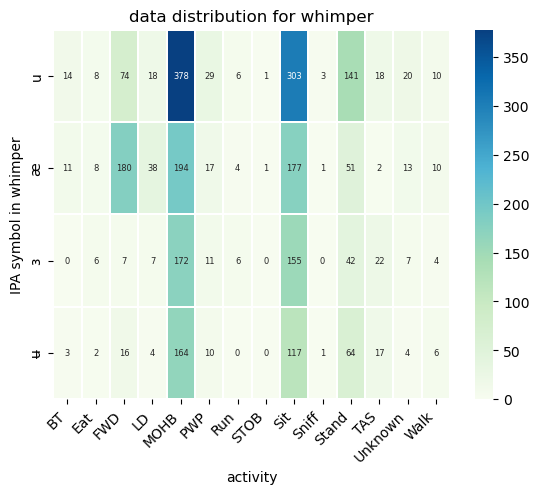
\includegraphics[width=0.9\textwidth]{images/symbol_whimper.png}
	\caption{Activity distribution of subwords for whimper.}
\label{fig:31}
\end{subfigure}
\begin{subfigure}[]{0.4\textwidth}
	\centering
	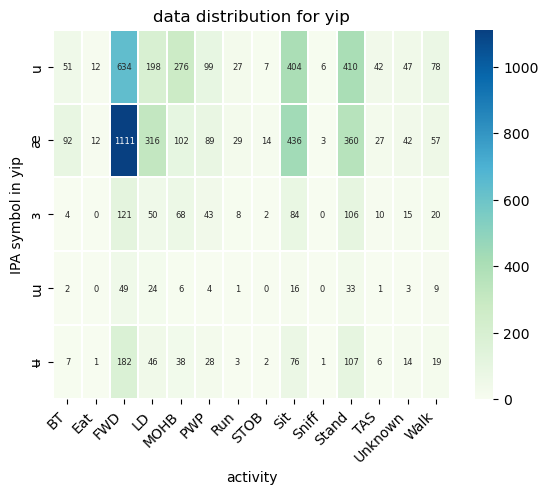
\includegraphics[width=0.9\textwidth]{images/symbol_yip.png}
	\caption{Activity distribution of subwords for yip.}
\label{fig:41}
\end{subfigure}

\begin{subfigure}[]{0.4\textwidth}
	\centering
	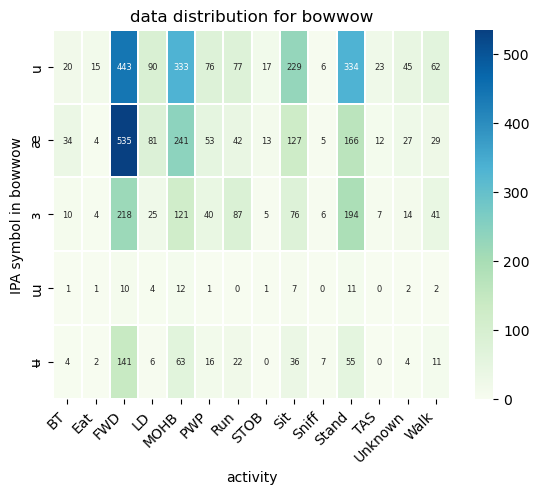
\includegraphics[width=0.9\textwidth]{images/symbol_bowwow.png}
	\caption{Activity distribution of subwords for bowwow.}
\label{fig:51}
\end{subfigure}
\begin{subfigure}[]{0.4\textwidth}
	\centering
	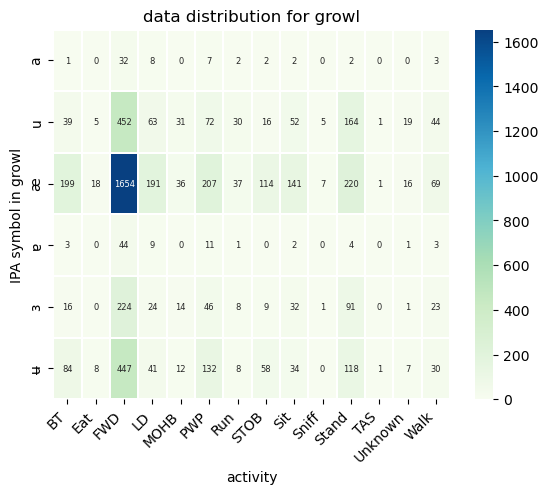
\includegraphics[width=0.9\textwidth]{images/symbol_growl.png}
	\caption{Activity distribution of subwords for growl.}
	\label{fig:61}
\end{subfigure}

\caption{Activity distribution of IPA symbol in word type.}
\label{fig:activity_symbol_word_type}
\end{figure*}


\section{Example scenario for acitivity and location}
In this section, we present picture examples to illustrate each activity and location for better understanding. ~\figref{fig:location_example} present the examples for locations. ~\figref{fig:activity_example} present the examples for activities. 

\begin{figure*}[h]
\centering
\begin{subfigure}[]{0.4\textwidth}
	\centering
	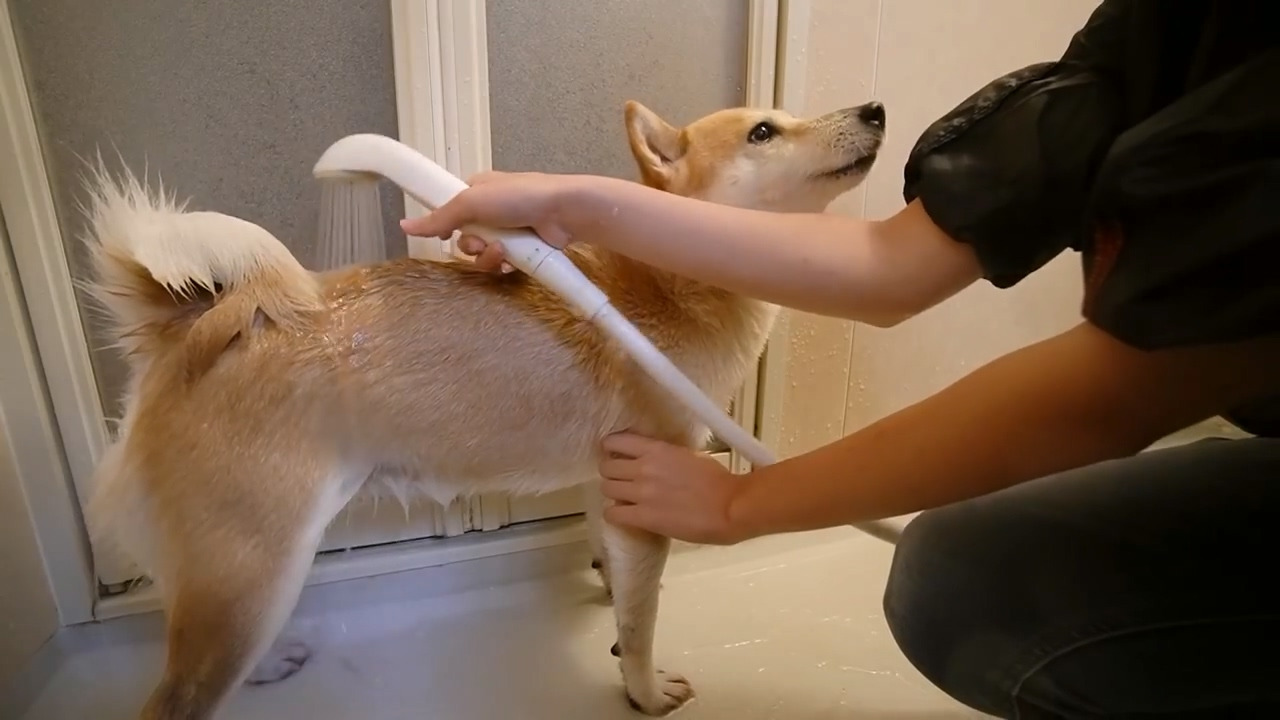
\includegraphics[width=0.9\textwidth]{images/bathroom.jpg}
	\caption{Bathroom example.}
	\label{fig:loc1}
\end{subfigure}
\begin{subfigure}[]{0.4\textwidth}
	\centering
	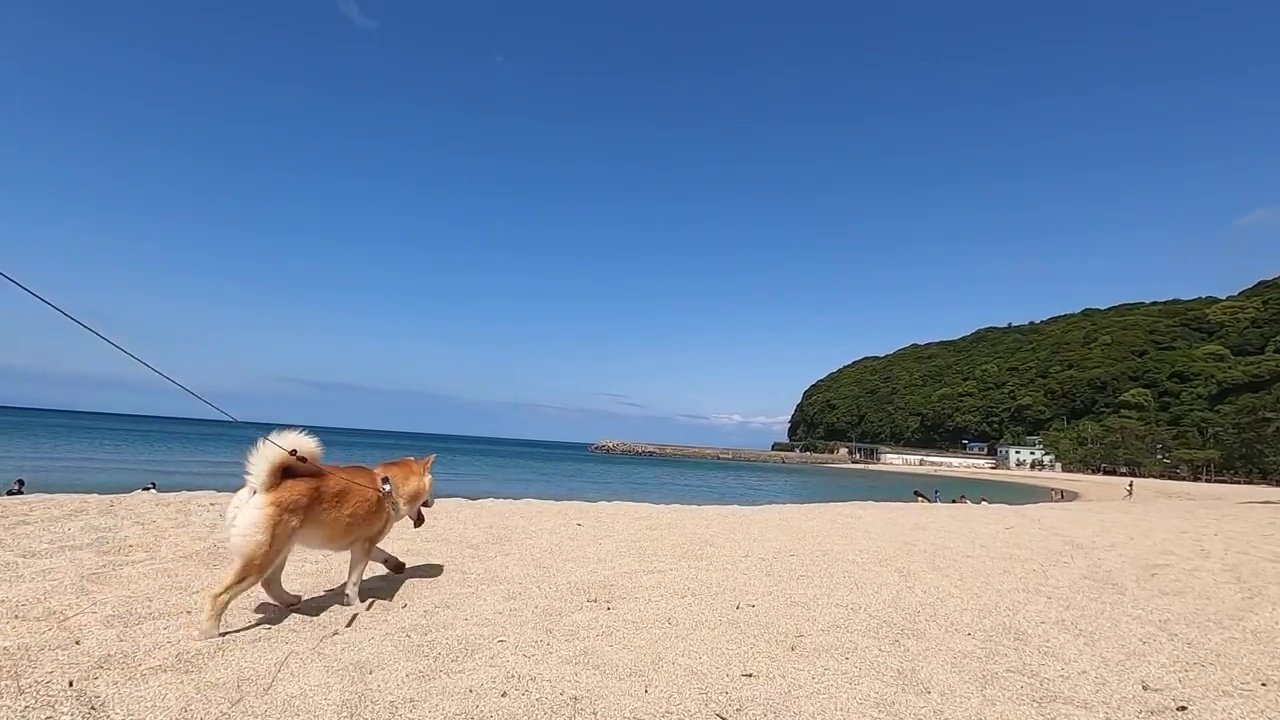
\includegraphics[width=0.9\textwidth]{images/beach.jpg}
	\caption{Beach example.}
	\label{fig:loc2}
\end{subfigure}

\begin{subfigure}[]{0.4\textwidth}
	\centering
	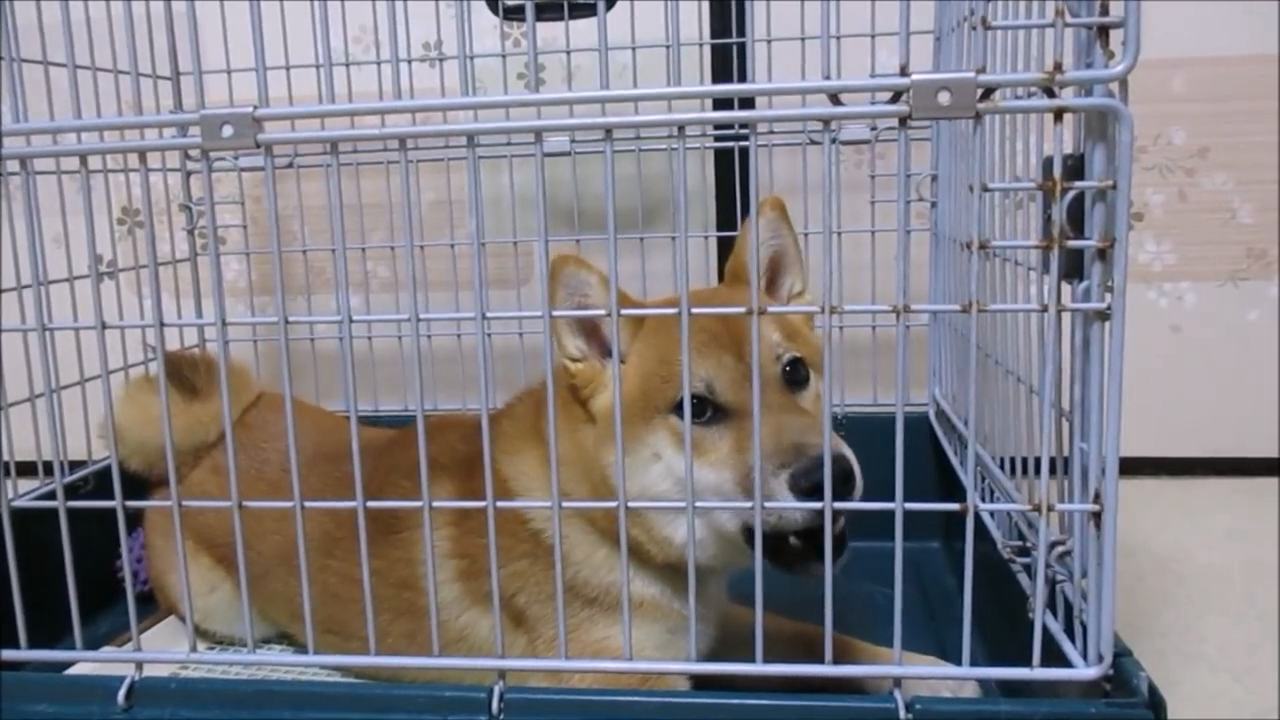
\includegraphics[width=0.9\textwidth]{images/cage.png}
	\caption{Cage example.}
\label{fig:loc3}
\end{subfigure}
\begin{subfigure}[]{0.4\textwidth}
	\centering
	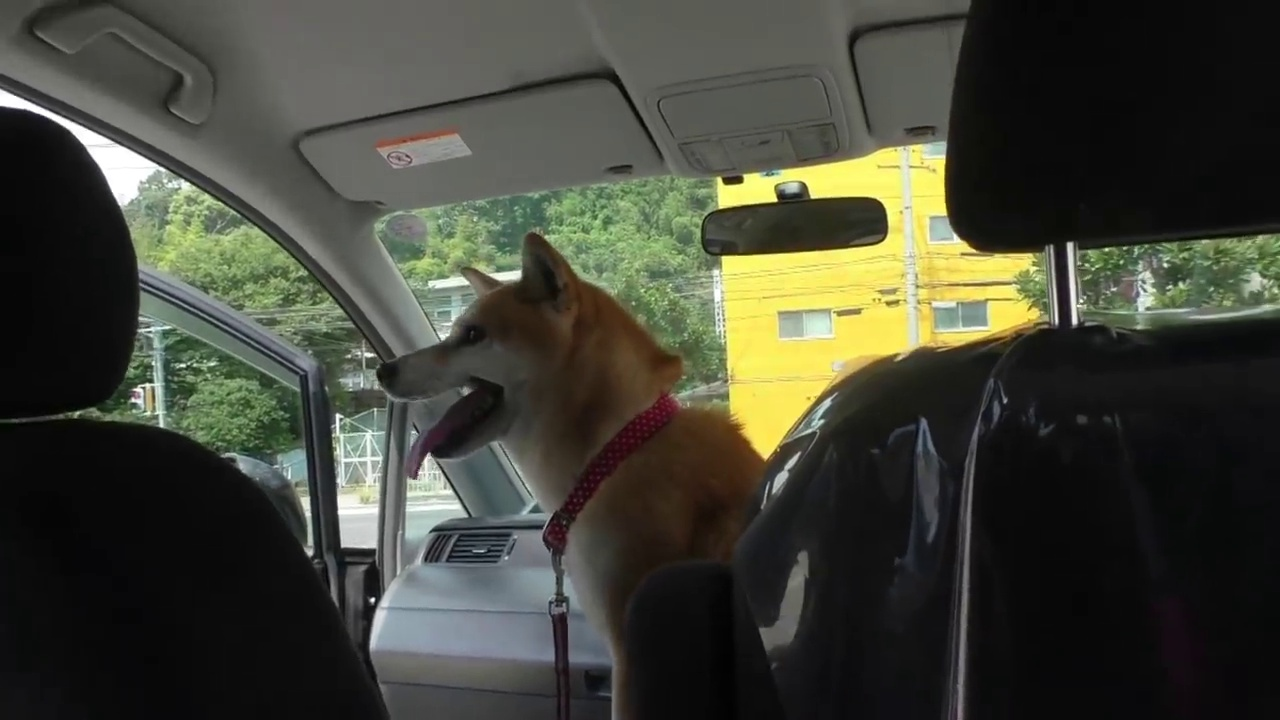
\includegraphics[width=0.9\textwidth]{images/cabin.jpg}
	\caption{Vehical cabin example.}
\label{fig:loc4}
\end{subfigure}

\begin{subfigure}[]{0.4\textwidth}
	\centering
	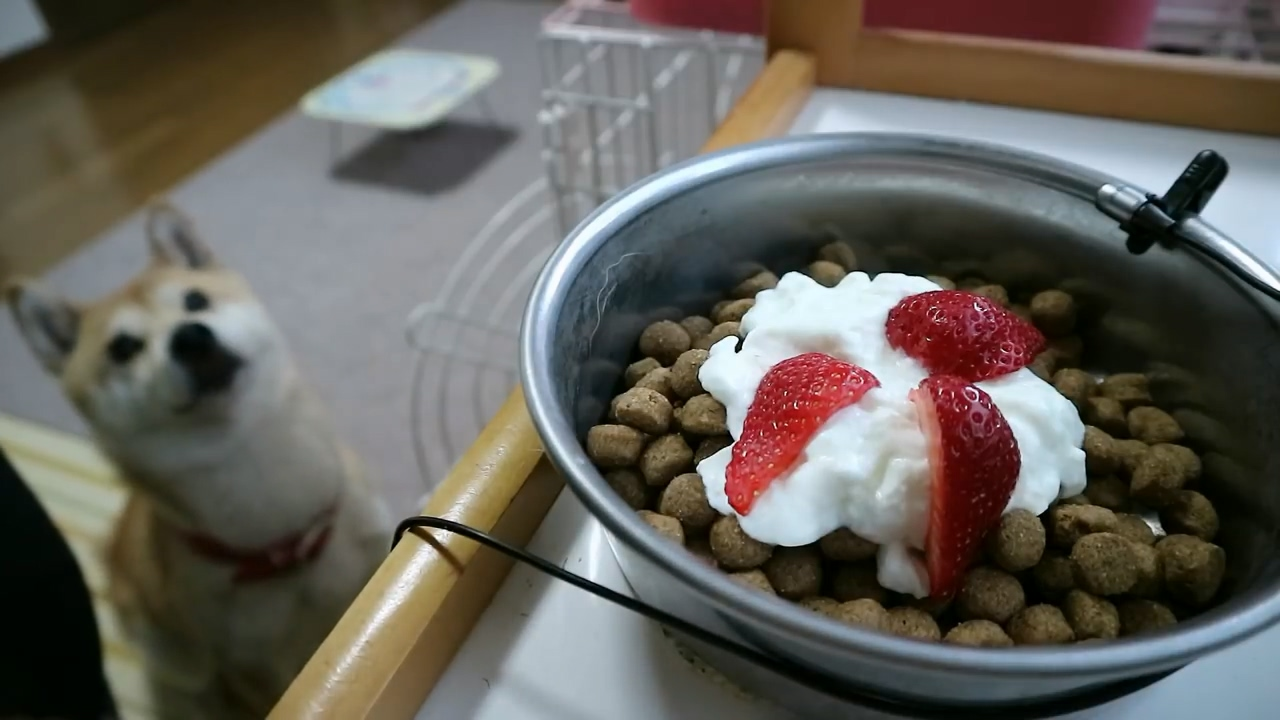
\includegraphics[width=0.9\textwidth]{images/foodnearby.jpg}
	\caption{Food nearby example.}
\label{fig:loc5}
\end{subfigure}
\begin{subfigure}[]{0.4\textwidth}
	\centering
	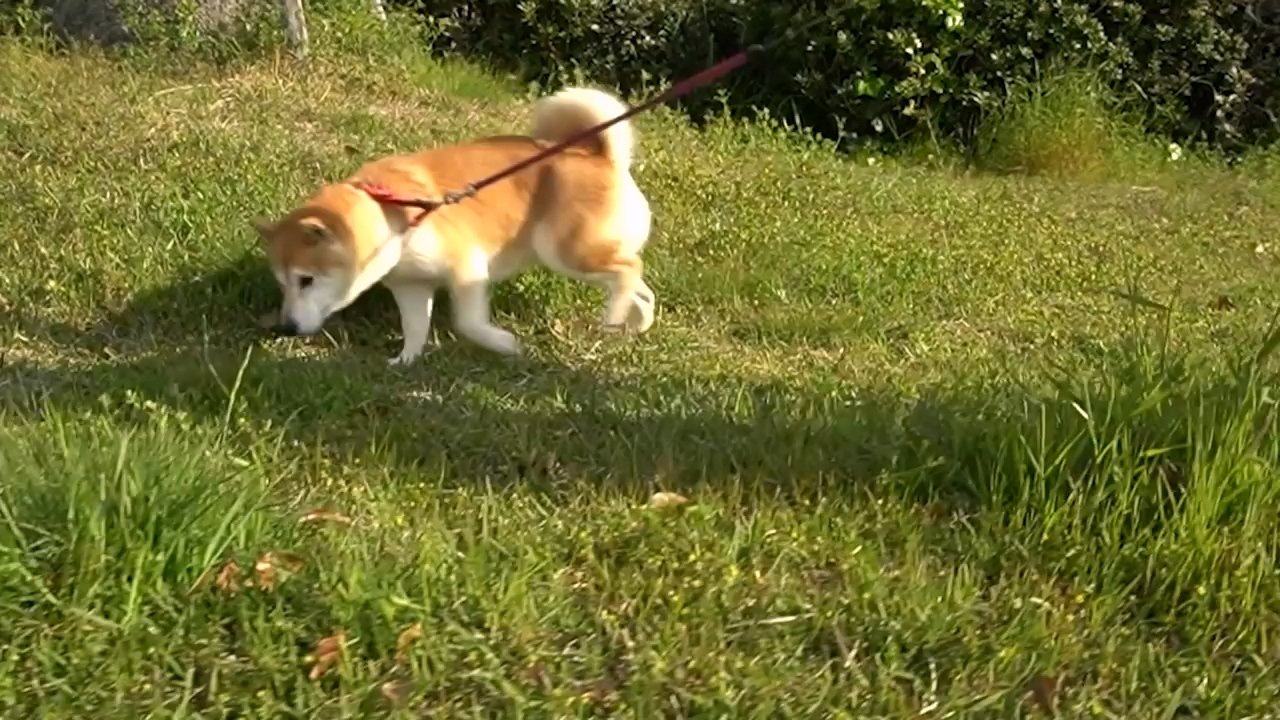
\includegraphics[width=0.9\textwidth]{images/grass.jpg}
	\caption{Grass example.}
	\label{fig:loc6}
\end{subfigure}

\begin{subfigure}[]{0.4\textwidth}
	\centering
	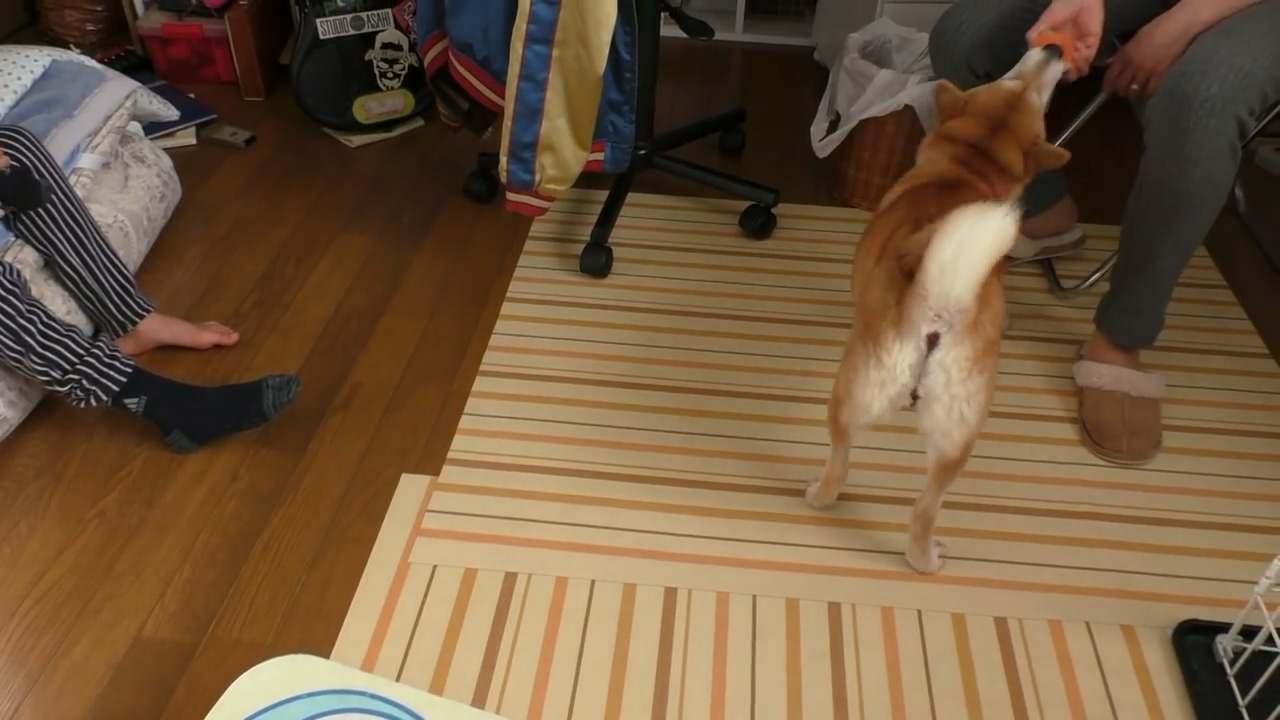
\includegraphics[width=0.9\textwidth]{images/livingroom.jpg}
	\caption{Living room example.}
\label{fig:loc7}
\end{subfigure}
\begin{subfigure}[]{0.4\textwidth}
	\centering
	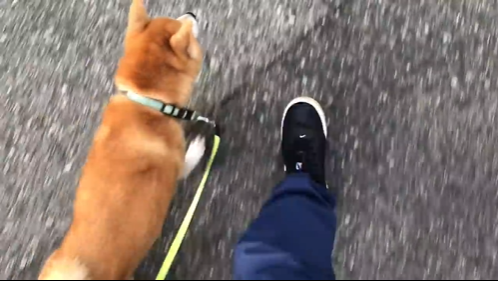
\includegraphics[width=0.9\textwidth]{images/road.png}
	\caption{Road example.}
	\label{fig:loc8}
\end{subfigure}

\begin{subfigure}[]{0.4\textwidth}
	\centering
	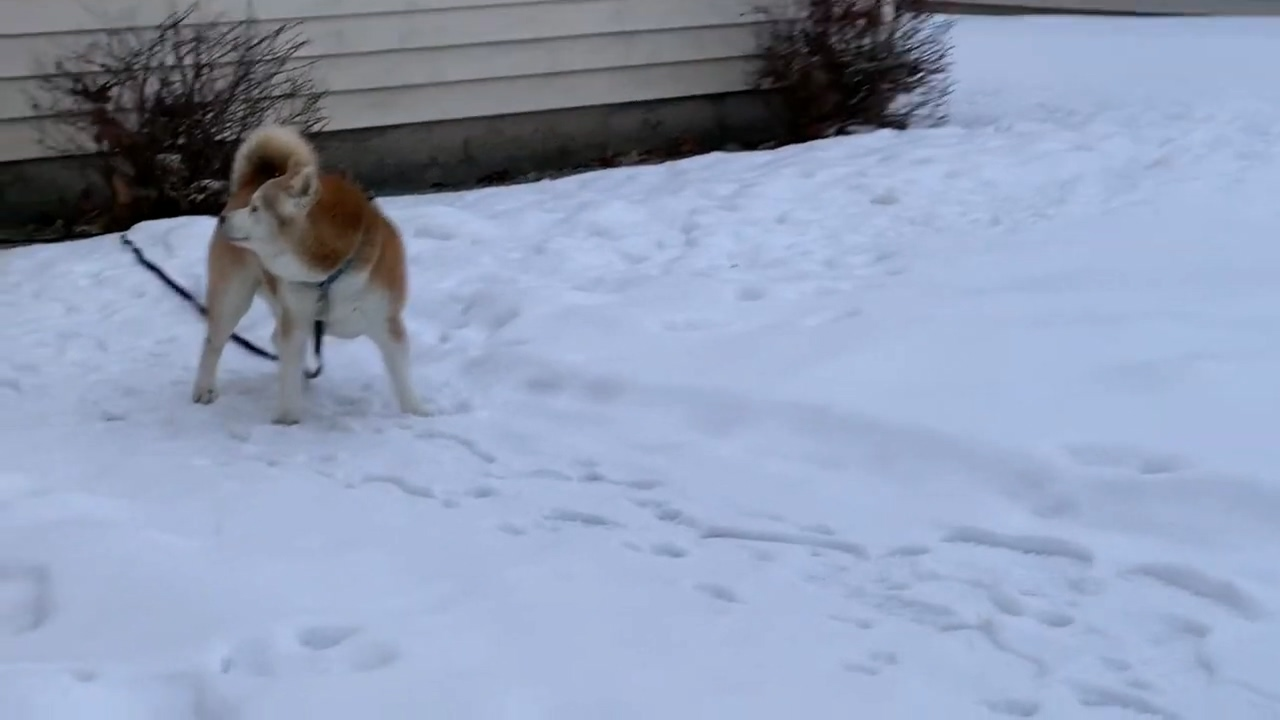
\includegraphics[width=0.9\textwidth]{images/snowfield.jpg}
	\caption{Snowfield example.}
\label{fig:loc9}
\end{subfigure}
\begin{subfigure}[]{0.4\textwidth}
	\centering
	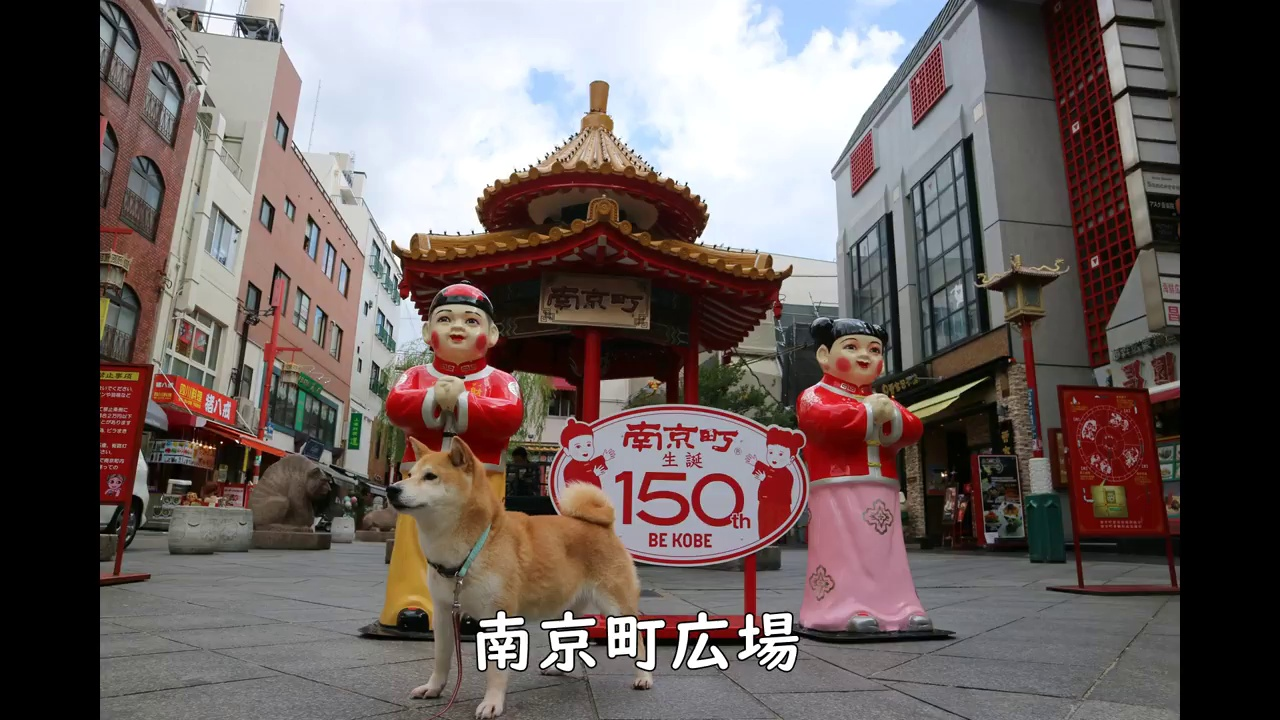
\includegraphics[width=0.9\textwidth]{images/square.jpg}
	\caption{Square example.}
	\label{fig:loc10}
\end{subfigure}

\begin{subfigure}[]{0.4\textwidth}
	\centering
	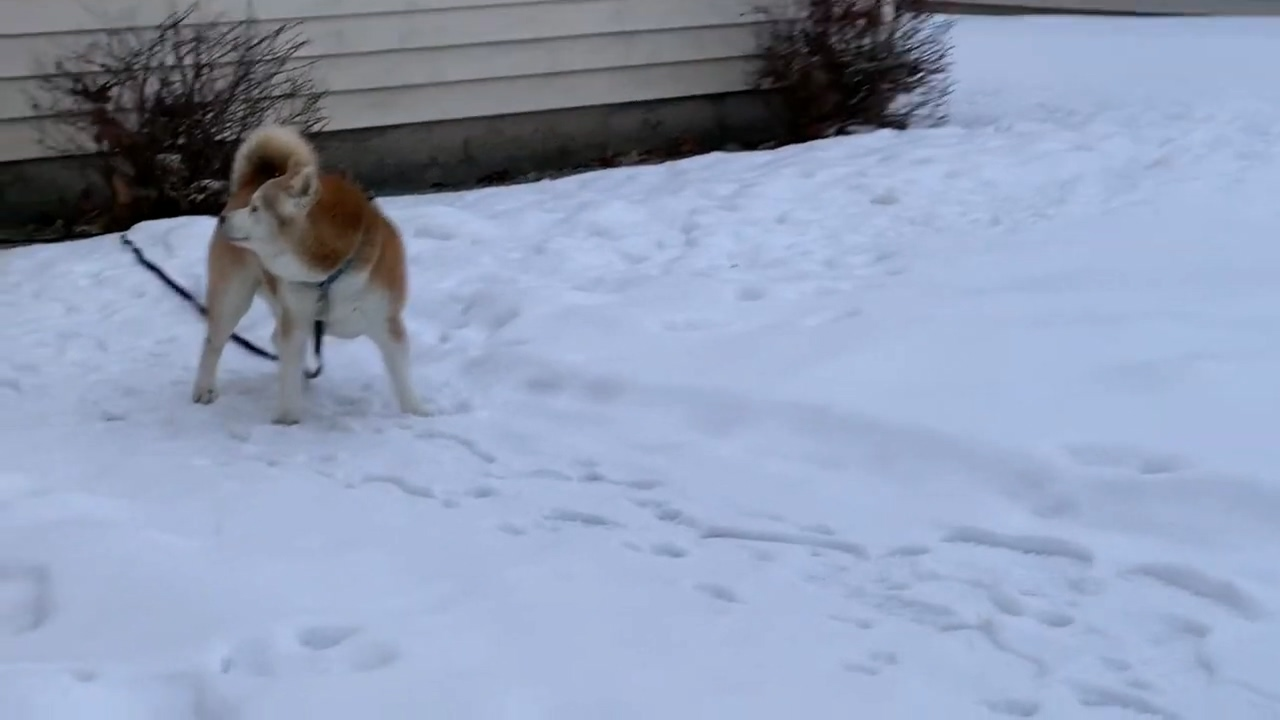
\includegraphics[width=0.9\textwidth]{images/snowfield.jpg}
	\caption{Snowfield example.}
\label{fig:loc11}
\end{subfigure}

\caption{Example for locations.}
\label{fig:location_example}
\end{figure*}


\begin{figure*}[h]
\centering
\begin{subfigure}[]{0.3\textwidth}
	\centering
	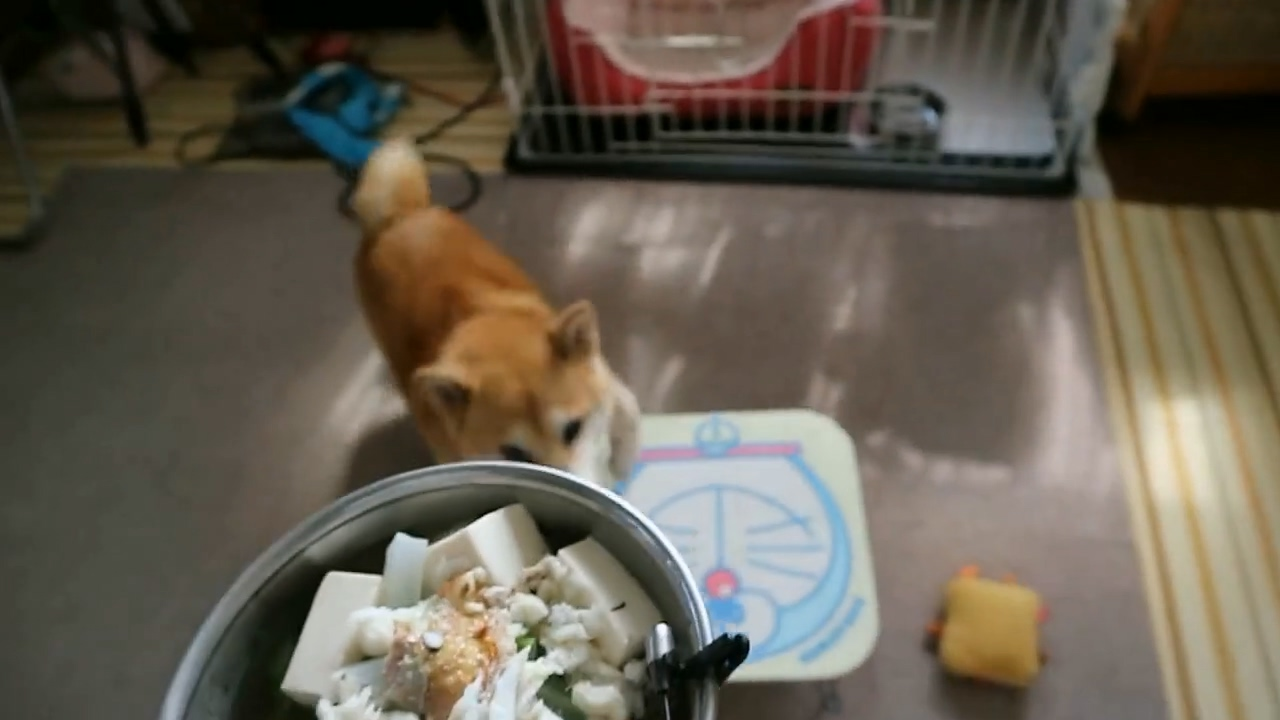
\includegraphics[width=0.9\textwidth]{images/mountorhump(beg).jpg}
	\caption{Mount or hump (beg) example.}
	\label{fig:act1}
\end{subfigure}
\begin{subfigure}[]{0.3\textwidth}
	\centering
	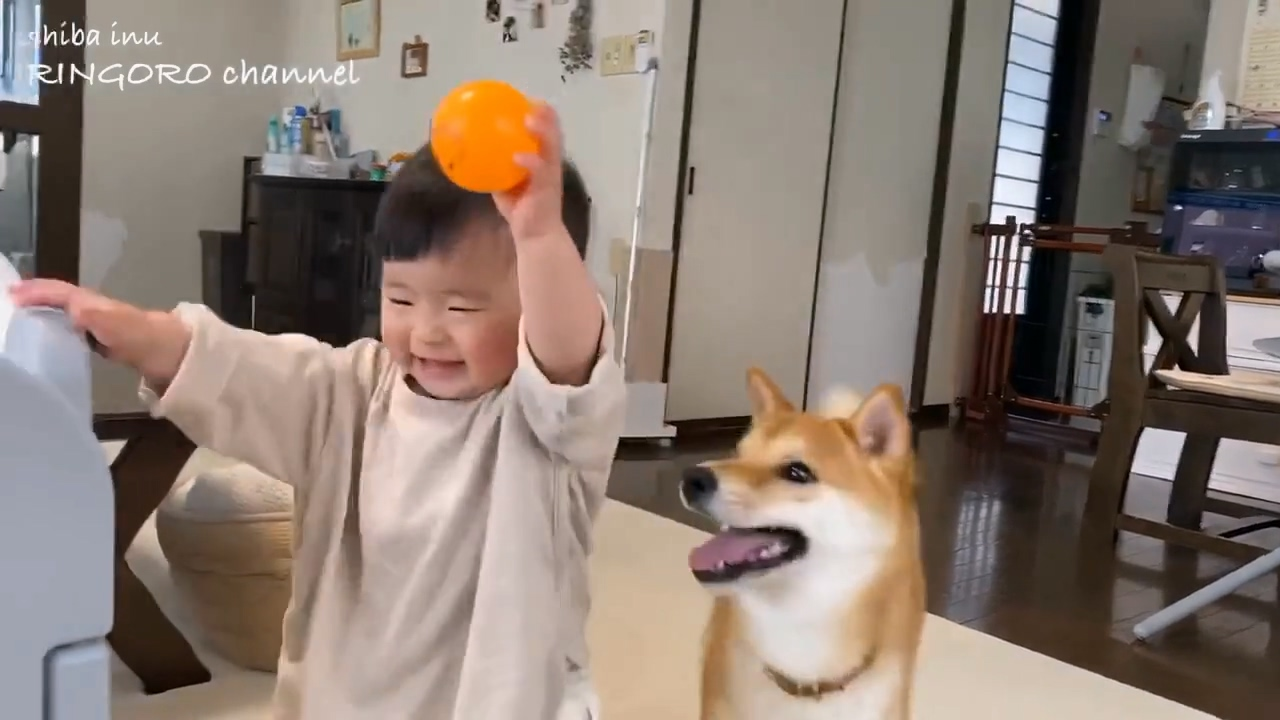
\includegraphics[width=0.9\textwidth]{images/playwithpeople.jpg}
	\caption{Play with people example.}
	\label{fig:act2}
\end{subfigure}
\begin{subfigure}[]{0.3\textwidth}
	\centering
	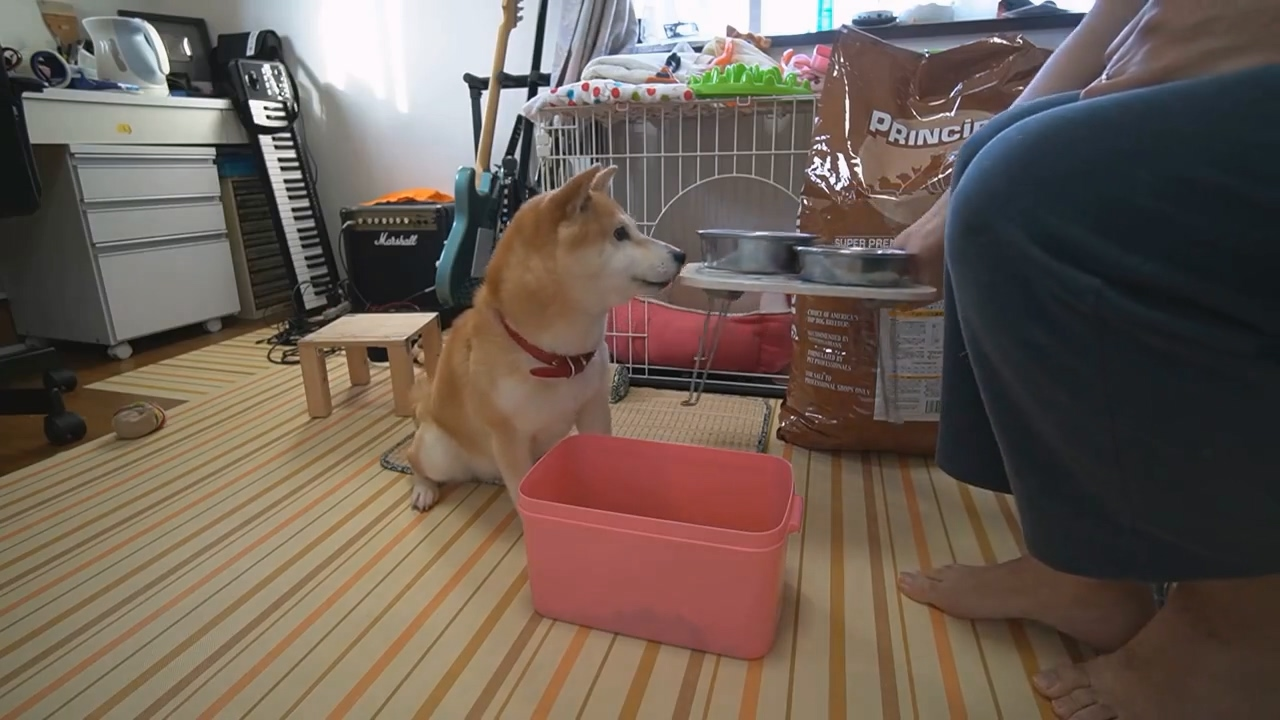
\includegraphics[width=0.9\textwidth]{images/sit.jpg}
	\caption{Sit example.}
\label{fig:act3}
\end{subfigure}

\begin{subfigure}[]{0.3\textwidth}
	\centering
	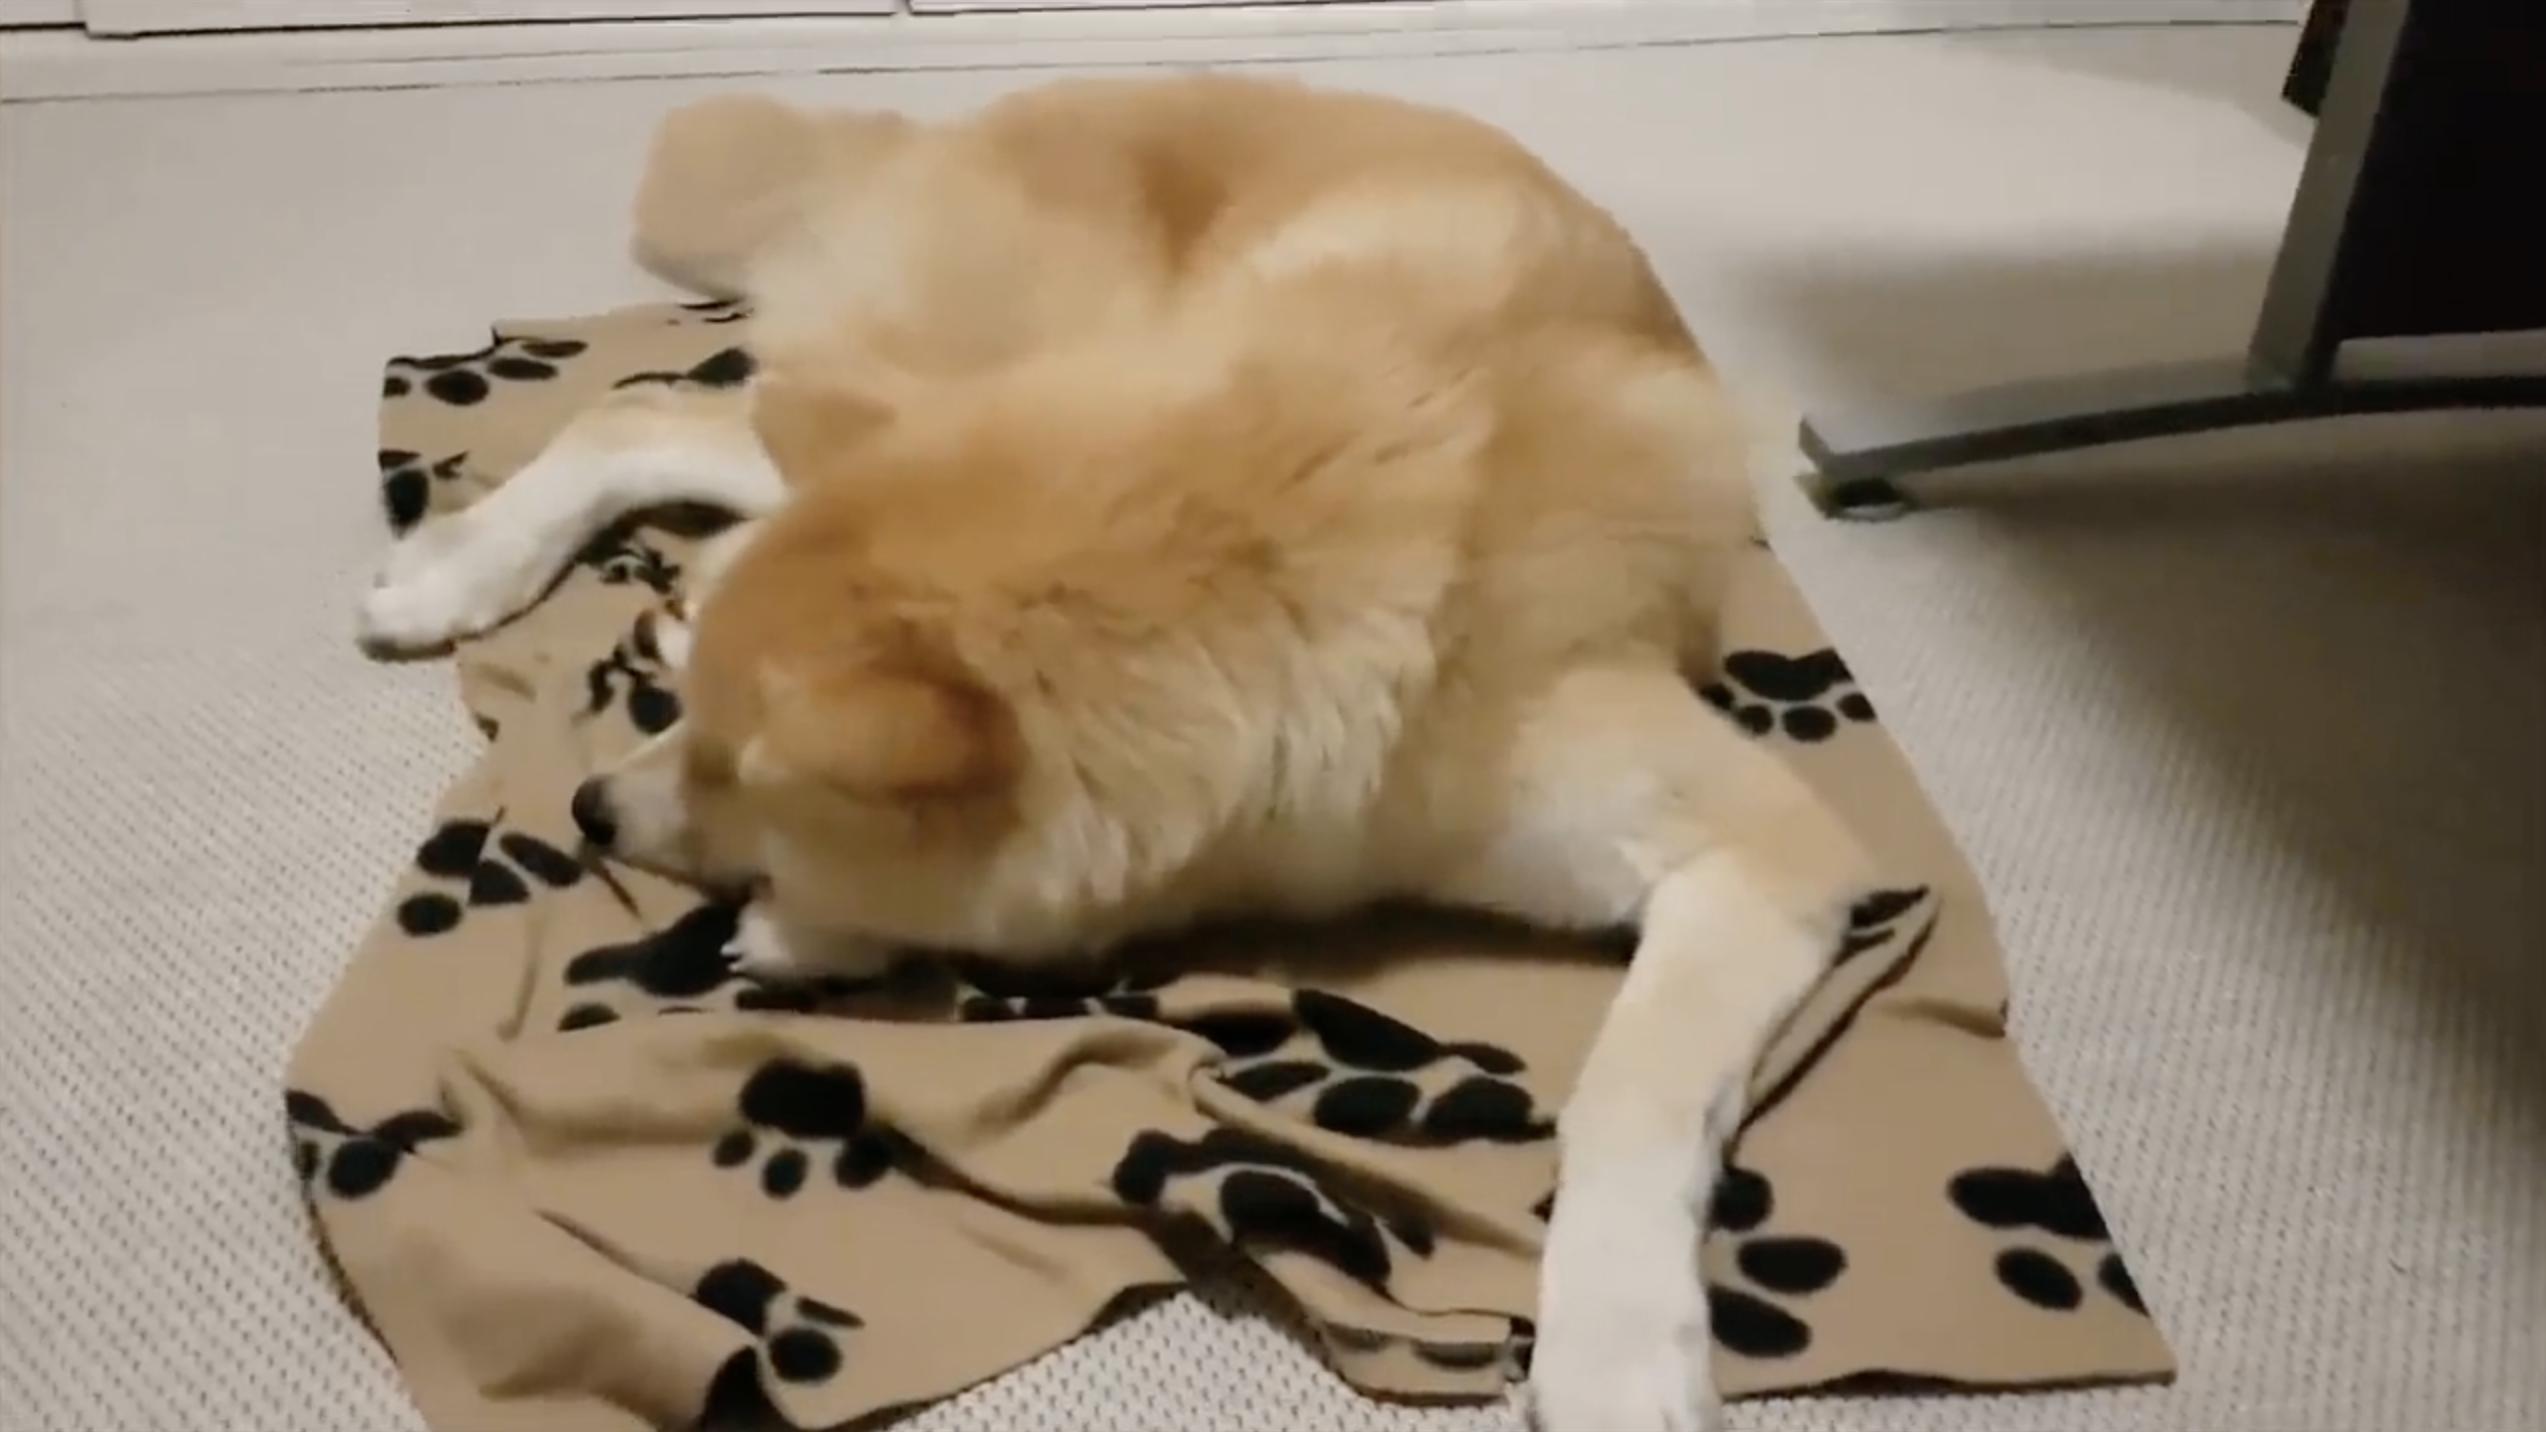
\includegraphics[width=0.9\textwidth]{images/laydown.png}
	\caption{Laydown example.}
\label{fig:act4}
\end{subfigure}
\begin{subfigure}[]{0.3\textwidth}
	\centering
	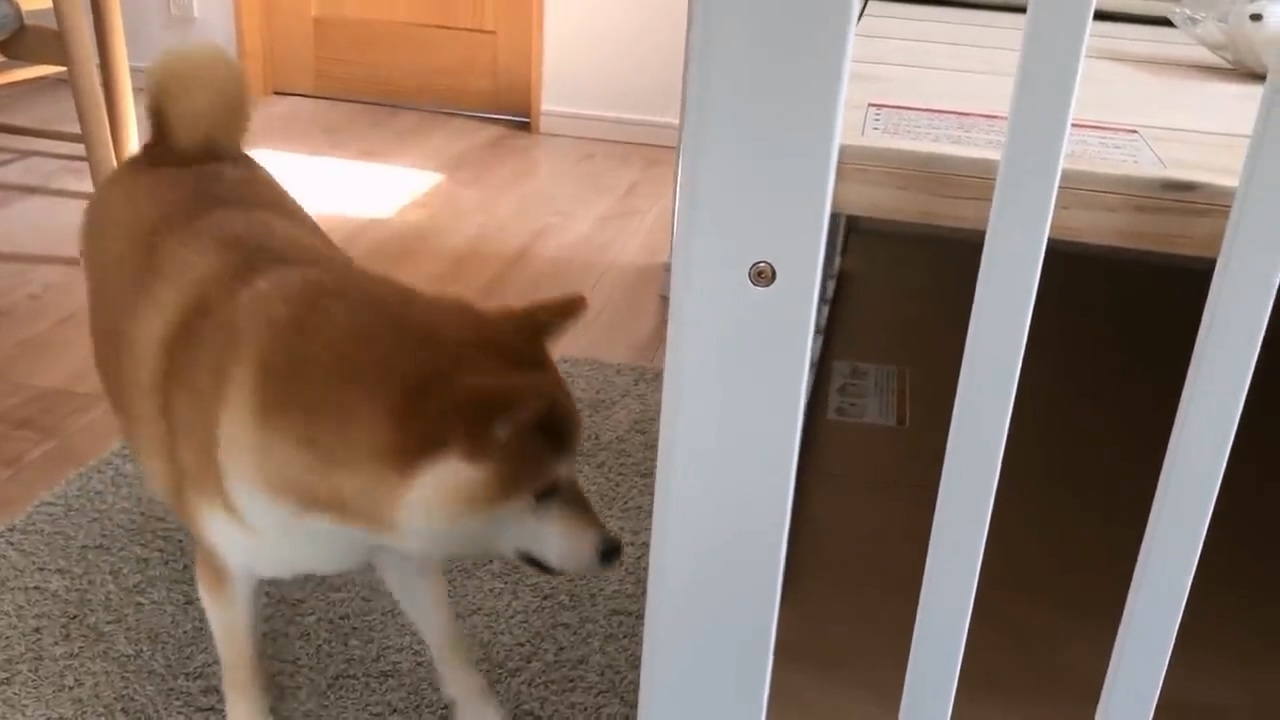
\includegraphics[width=0.9\textwidth]{images/walk.jpg}
	\caption{Walk example.}
\label{fig:act5}
\end{subfigure}
\begin{subfigure}[]{0.3\textwidth}
	\centering
	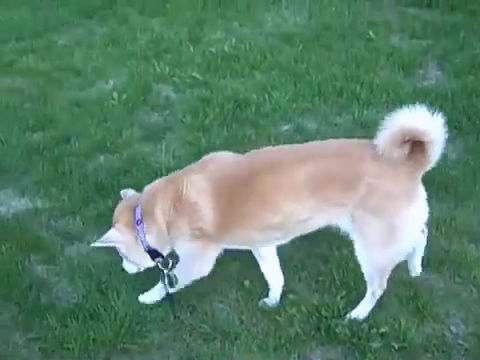
\includegraphics[width=0.9\textwidth]{images/sniff.jpg}
	\caption{Sniff example.}
	\label{fig:act6}
\end{subfigure}

\begin{subfigure}[]{0.3\textwidth}
	\centering
	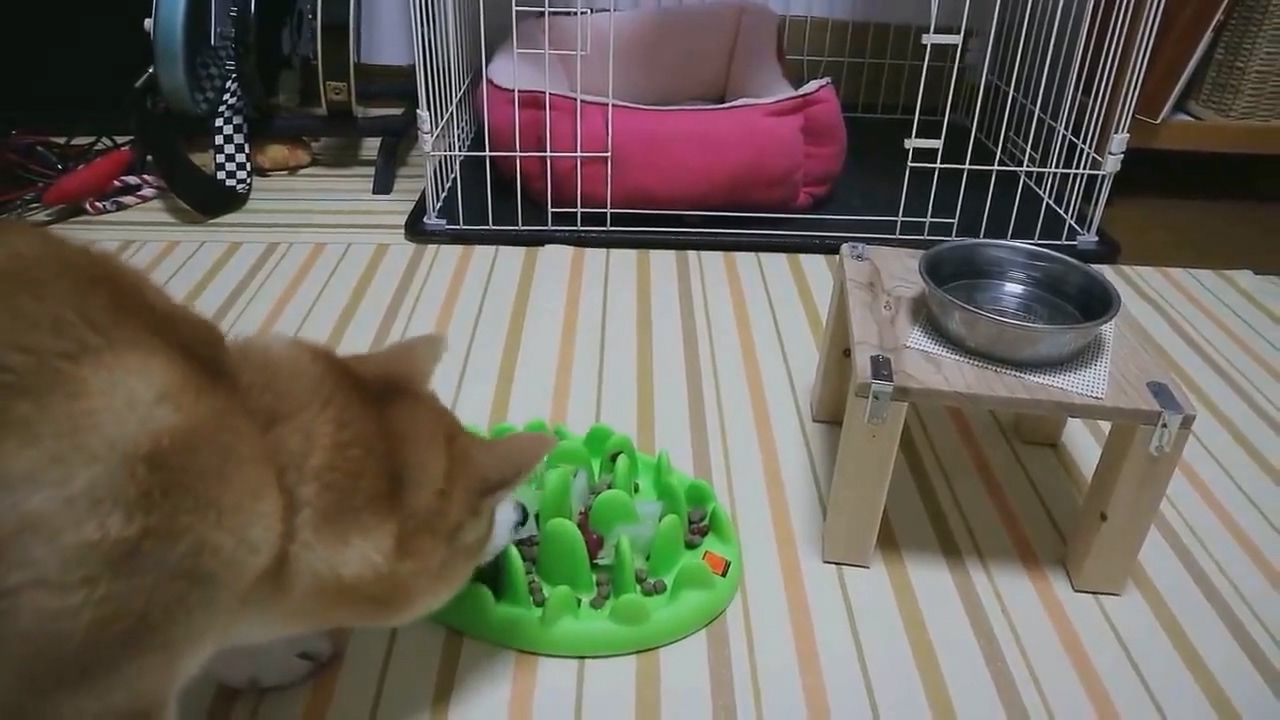
\includegraphics[width=0.9\textwidth]{images/eat.jpg}
	\caption{Eat example.}
\label{fig:act7}
\end{subfigure}
\begin{subfigure}[]{0.3\textwidth}
	\centering
	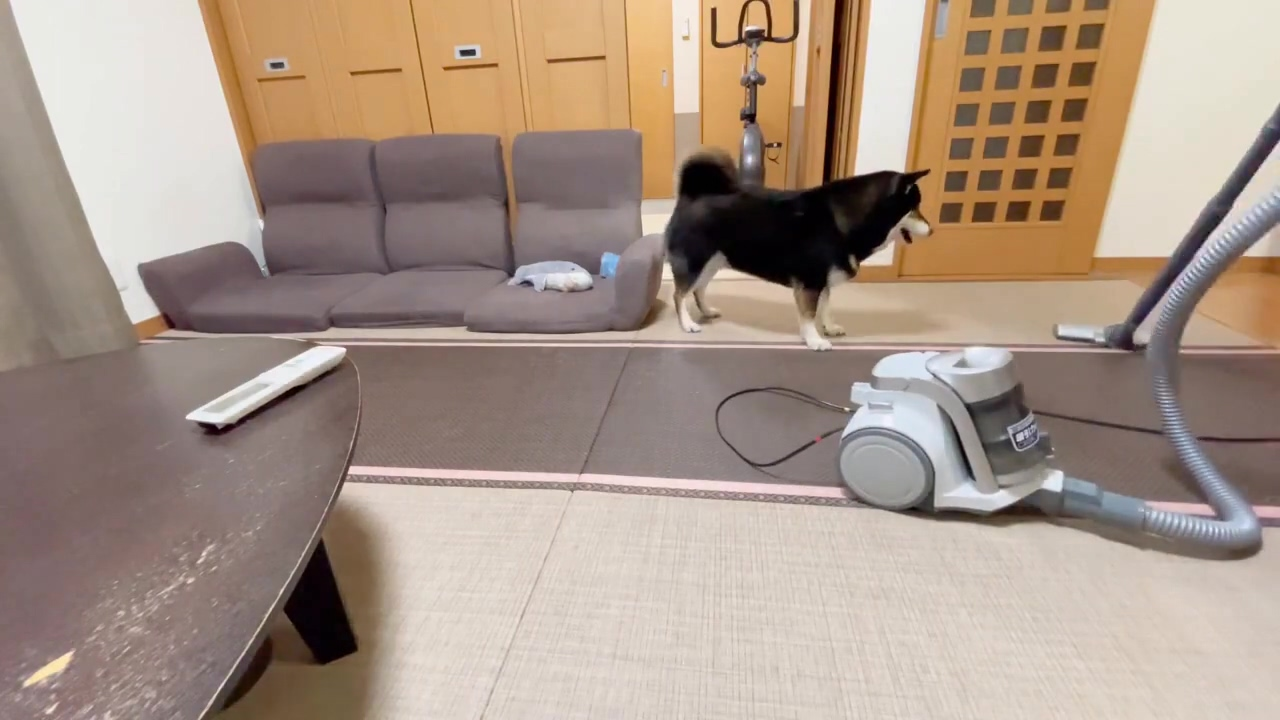
\includegraphics[width=0.9\textwidth]{images/stand.jpg}
	\caption{Stand example.}
	\label{fig:act8}
\end{subfigure}
\begin{subfigure}[]{0.3\textwidth}
	\centering
	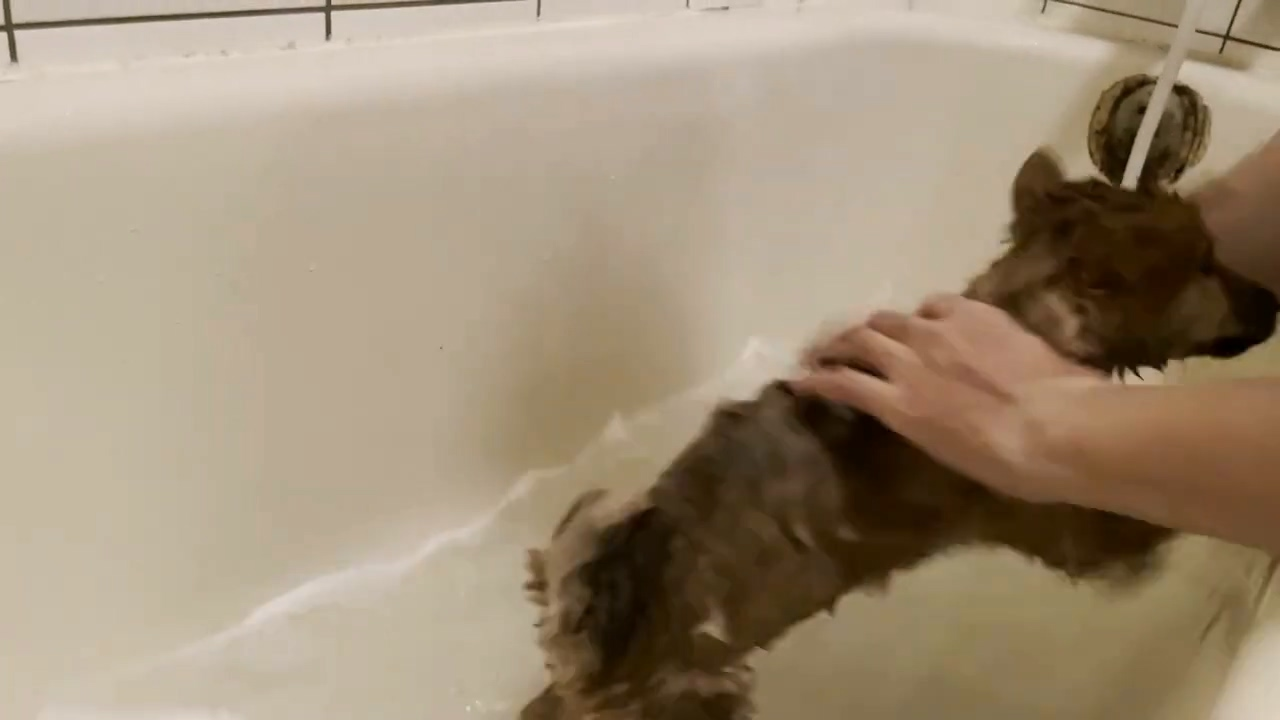
\includegraphics[width=0.9\textwidth]{images/takeashower.jpg}
	\caption{Take a shower example.}
\label{fig:act9}
\end{subfigure}

\begin{subfigure}[]{0.3\textwidth}
	\centering
	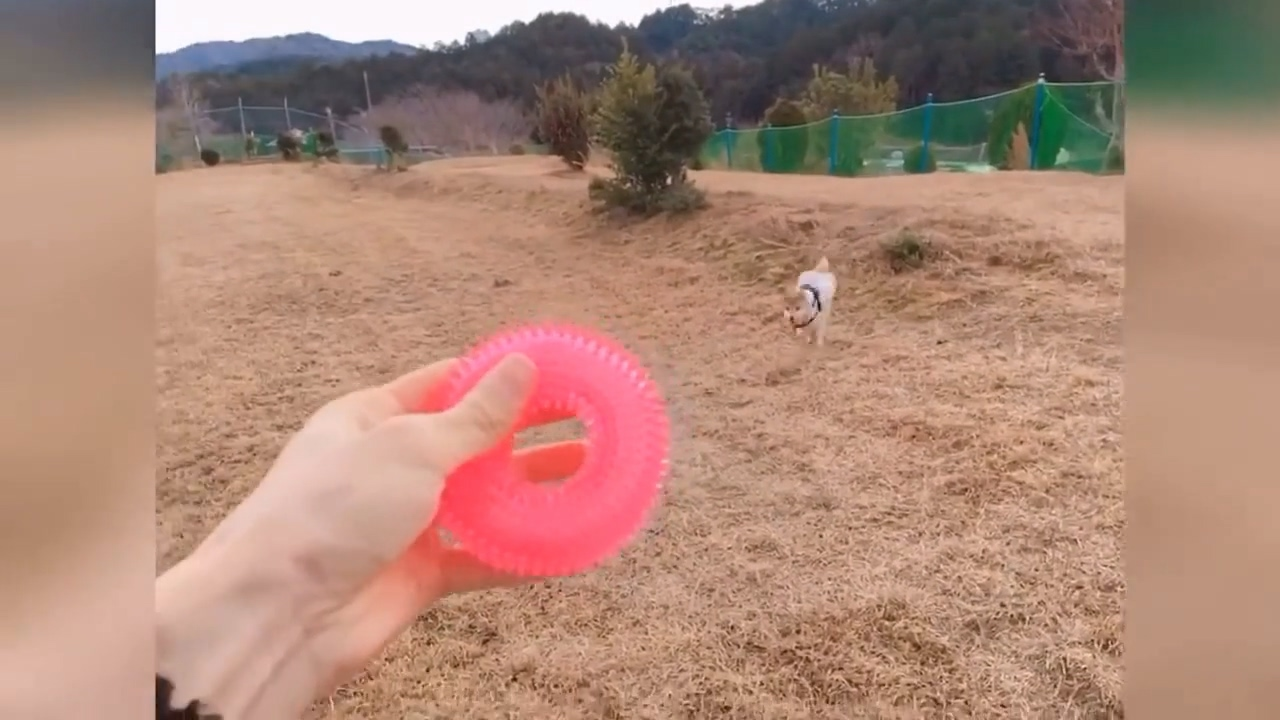
\includegraphics[width=0.9\textwidth]{images/run.jpg}
	\caption{Run example.}
	\label{fig:act10}
\end{subfigure}
\begin{subfigure}[]{0.3\textwidth}
	\centering
	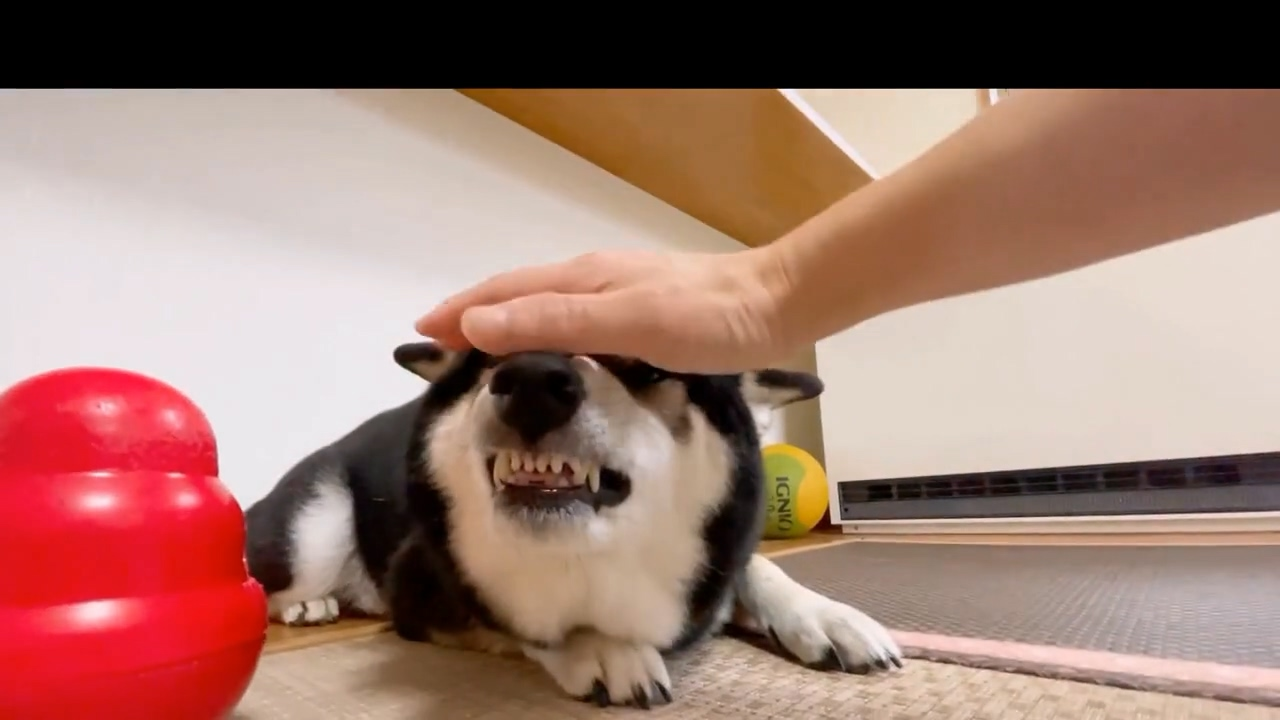
\includegraphics[width=0.9\textwidth]{images/betouched.jpg}
	\caption{Be touched example.}
\label{fig:act11}
\end{subfigure}
\begin{subfigure}[]{0.3\textwidth}
	\centering
	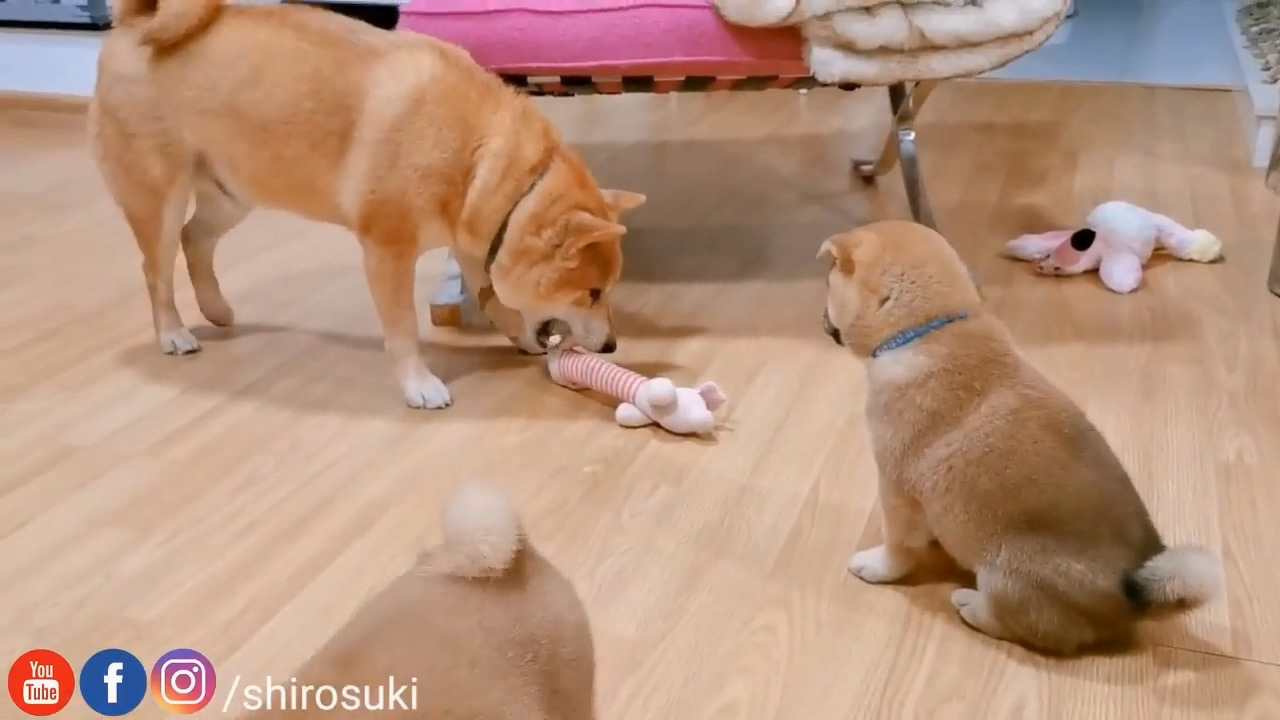
\includegraphics[width=0.9\textwidth]{images/showteethorbit.jpg}
	\caption{Show teech or bit example.}
\label{fig:act12}
\end{subfigure}

\begin{subfigure}[]{0.3\textwidth}
	\centering
	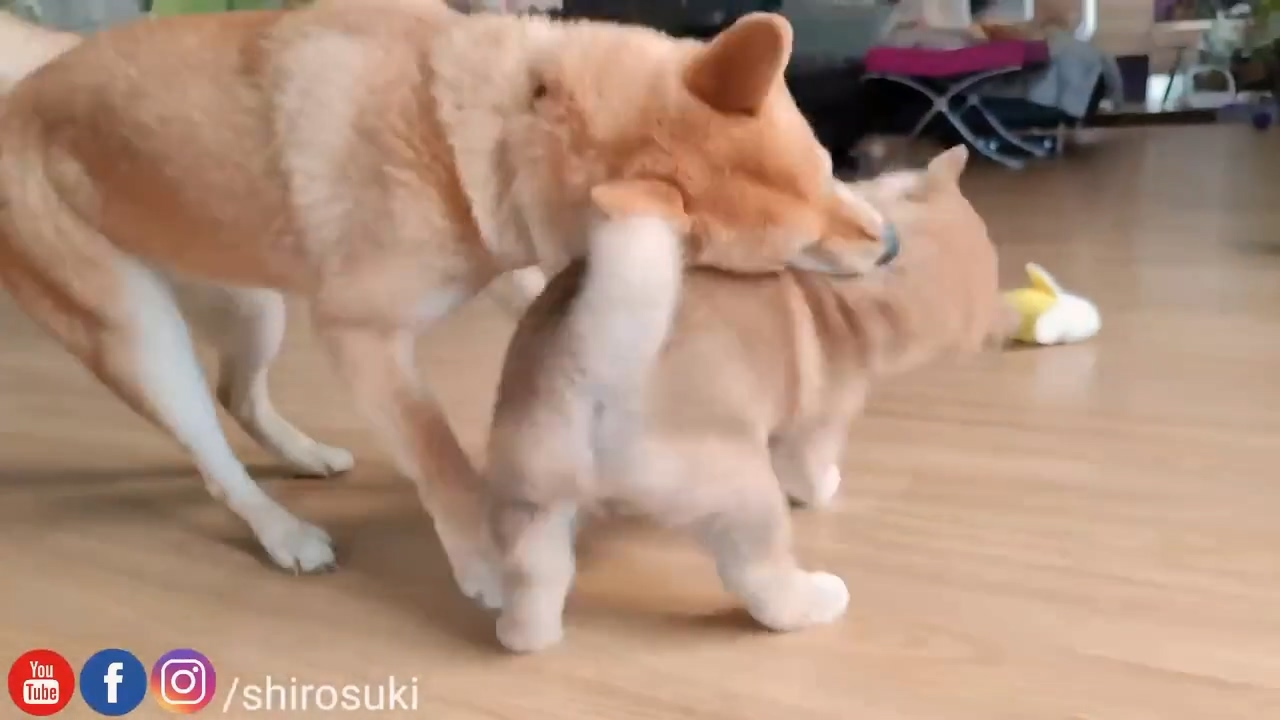
\includegraphics[width=0.9\textwidth]{images/fightwithdogs.jpg}
	\caption{Fight with dogs example.}
	\label{fig:act13}
\end{subfigure}



\caption{Example for activities.}
\label{fig:activity_example}
\end{figure*}

\end{document}
